% Options for packages loaded elsewhere
\PassOptionsToPackage{unicode}{hyperref}
\PassOptionsToPackage{hyphens}{url}
%
\documentclass[
]{article}
\title{ED 216B: Lab 1 - Introduction to Mplus and RStudio}
\usepackage{etoolbox}
\makeatletter
\providecommand{\subtitle}[1]{% add subtitle to \maketitle
  \apptocmd{\@title}{\par {\large #1 \par}}{}{}
}
\makeatother
\subtitle{Winter 2022}
\author{TA: Dina Arch}
\date{1/3/2022}

\usepackage{amsmath,amssymb}
\usepackage{lmodern}
\usepackage{iftex}
\ifPDFTeX
  \usepackage[T1]{fontenc}
  \usepackage[utf8]{inputenc}
  \usepackage{textcomp} % provide euro and other symbols
\else % if luatex or xetex
  \usepackage{unicode-math}
  \defaultfontfeatures{Scale=MatchLowercase}
  \defaultfontfeatures[\rmfamily]{Ligatures=TeX,Scale=1}
\fi
% Use upquote if available, for straight quotes in verbatim environments
\IfFileExists{upquote.sty}{\usepackage{upquote}}{}
\IfFileExists{microtype.sty}{% use microtype if available
  \usepackage[]{microtype}
  \UseMicrotypeSet[protrusion]{basicmath} % disable protrusion for tt fonts
}{}
\makeatletter
\@ifundefined{KOMAClassName}{% if non-KOMA class
  \IfFileExists{parskip.sty}{%
    \usepackage{parskip}
  }{% else
    \setlength{\parindent}{0pt}
    \setlength{\parskip}{6pt plus 2pt minus 1pt}}
}{% if KOMA class
  \KOMAoptions{parskip=half}}
\makeatother
\usepackage{xcolor}
\IfFileExists{xurl.sty}{\usepackage{xurl}}{} % add URL line breaks if available
\IfFileExists{bookmark.sty}{\usepackage{bookmark}}{\usepackage{hyperref}}
\hypersetup{
  pdftitle={ED 216B: Lab 1 - Introduction to Mplus and RStudio},
  pdfauthor={TA: Dina Arch},
  hidelinks,
  pdfcreator={LaTeX via pandoc}}
\urlstyle{same} % disable monospaced font for URLs
\usepackage[margin=1in]{geometry}
\usepackage{color}
\usepackage{fancyvrb}
\newcommand{\VerbBar}{|}
\newcommand{\VERB}{\Verb[commandchars=\\\{\}]}
\DefineVerbatimEnvironment{Highlighting}{Verbatim}{commandchars=\\\{\}}
% Add ',fontsize=\small' for more characters per line
\usepackage{framed}
\definecolor{shadecolor}{RGB}{248,248,248}
\newenvironment{Shaded}{\begin{snugshade}}{\end{snugshade}}
\newcommand{\AlertTok}[1]{\textcolor[rgb]{0.94,0.16,0.16}{#1}}
\newcommand{\AnnotationTok}[1]{\textcolor[rgb]{0.56,0.35,0.01}{\textbf{\textit{#1}}}}
\newcommand{\AttributeTok}[1]{\textcolor[rgb]{0.77,0.63,0.00}{#1}}
\newcommand{\BaseNTok}[1]{\textcolor[rgb]{0.00,0.00,0.81}{#1}}
\newcommand{\BuiltInTok}[1]{#1}
\newcommand{\CharTok}[1]{\textcolor[rgb]{0.31,0.60,0.02}{#1}}
\newcommand{\CommentTok}[1]{\textcolor[rgb]{0.56,0.35,0.01}{\textit{#1}}}
\newcommand{\CommentVarTok}[1]{\textcolor[rgb]{0.56,0.35,0.01}{\textbf{\textit{#1}}}}
\newcommand{\ConstantTok}[1]{\textcolor[rgb]{0.00,0.00,0.00}{#1}}
\newcommand{\ControlFlowTok}[1]{\textcolor[rgb]{0.13,0.29,0.53}{\textbf{#1}}}
\newcommand{\DataTypeTok}[1]{\textcolor[rgb]{0.13,0.29,0.53}{#1}}
\newcommand{\DecValTok}[1]{\textcolor[rgb]{0.00,0.00,0.81}{#1}}
\newcommand{\DocumentationTok}[1]{\textcolor[rgb]{0.56,0.35,0.01}{\textbf{\textit{#1}}}}
\newcommand{\ErrorTok}[1]{\textcolor[rgb]{0.64,0.00,0.00}{\textbf{#1}}}
\newcommand{\ExtensionTok}[1]{#1}
\newcommand{\FloatTok}[1]{\textcolor[rgb]{0.00,0.00,0.81}{#1}}
\newcommand{\FunctionTok}[1]{\textcolor[rgb]{0.00,0.00,0.00}{#1}}
\newcommand{\ImportTok}[1]{#1}
\newcommand{\InformationTok}[1]{\textcolor[rgb]{0.56,0.35,0.01}{\textbf{\textit{#1}}}}
\newcommand{\KeywordTok}[1]{\textcolor[rgb]{0.13,0.29,0.53}{\textbf{#1}}}
\newcommand{\NormalTok}[1]{#1}
\newcommand{\OperatorTok}[1]{\textcolor[rgb]{0.81,0.36,0.00}{\textbf{#1}}}
\newcommand{\OtherTok}[1]{\textcolor[rgb]{0.56,0.35,0.01}{#1}}
\newcommand{\PreprocessorTok}[1]{\textcolor[rgb]{0.56,0.35,0.01}{\textit{#1}}}
\newcommand{\RegionMarkerTok}[1]{#1}
\newcommand{\SpecialCharTok}[1]{\textcolor[rgb]{0.00,0.00,0.00}{#1}}
\newcommand{\SpecialStringTok}[1]{\textcolor[rgb]{0.31,0.60,0.02}{#1}}
\newcommand{\StringTok}[1]{\textcolor[rgb]{0.31,0.60,0.02}{#1}}
\newcommand{\VariableTok}[1]{\textcolor[rgb]{0.00,0.00,0.00}{#1}}
\newcommand{\VerbatimStringTok}[1]{\textcolor[rgb]{0.31,0.60,0.02}{#1}}
\newcommand{\WarningTok}[1]{\textcolor[rgb]{0.56,0.35,0.01}{\textbf{\textit{#1}}}}
\usepackage{longtable,booktabs,array}
\usepackage{calc} % for calculating minipage widths
% Correct order of tables after \paragraph or \subparagraph
\usepackage{etoolbox}
\makeatletter
\patchcmd\longtable{\par}{\if@noskipsec\mbox{}\fi\par}{}{}
\makeatother
% Allow footnotes in longtable head/foot
\IfFileExists{footnotehyper.sty}{\usepackage{footnotehyper}}{\usepackage{footnote}}
\makesavenoteenv{longtable}
\usepackage{graphicx}
\makeatletter
\def\maxwidth{\ifdim\Gin@nat@width>\linewidth\linewidth\else\Gin@nat@width\fi}
\def\maxheight{\ifdim\Gin@nat@height>\textheight\textheight\else\Gin@nat@height\fi}
\makeatother
% Scale images if necessary, so that they will not overflow the page
% margins by default, and it is still possible to overwrite the defaults
% using explicit options in \includegraphics[width, height, ...]{}
\setkeys{Gin}{width=\maxwidth,height=\maxheight,keepaspectratio}
% Set default figure placement to htbp
\makeatletter
\def\fps@figure{htbp}
\makeatother
\setlength{\emergencystretch}{3em} % prevent overfull lines
\providecommand{\tightlist}{%
  \setlength{\itemsep}{0pt}\setlength{\parskip}{0pt}}
\setcounter{secnumdepth}{-\maxdimen} % remove section numbering
\ifLuaTeX
  \usepackage{selnolig}  % disable illegal ligatures
\fi

\begin{document}
\maketitle

{
\setcounter{tocdepth}{2}
\tableofcontents
}
For the part 1 of our lab, we will first walk through how to run basic
descriptive statistics using only Mplus. Then in the in the second part,
we will use an R package called \texttt{MplusAutomation} to run the same
analysis as part 1, only this time using only RStudio.

\hypertarget{part-1-introduction-to-mplus}{%
\subsection{\texorpdfstring{\underline{PART 1}: Introduction to
Mplus}{PART 1: Introduction to Mplus}}\label{part-1-introduction-to-mplus}}

\hypertarget{step-1-open-appstream}{%
\subsubsection{Step 1: Open AppStream}\label{step-1-open-appstream}}

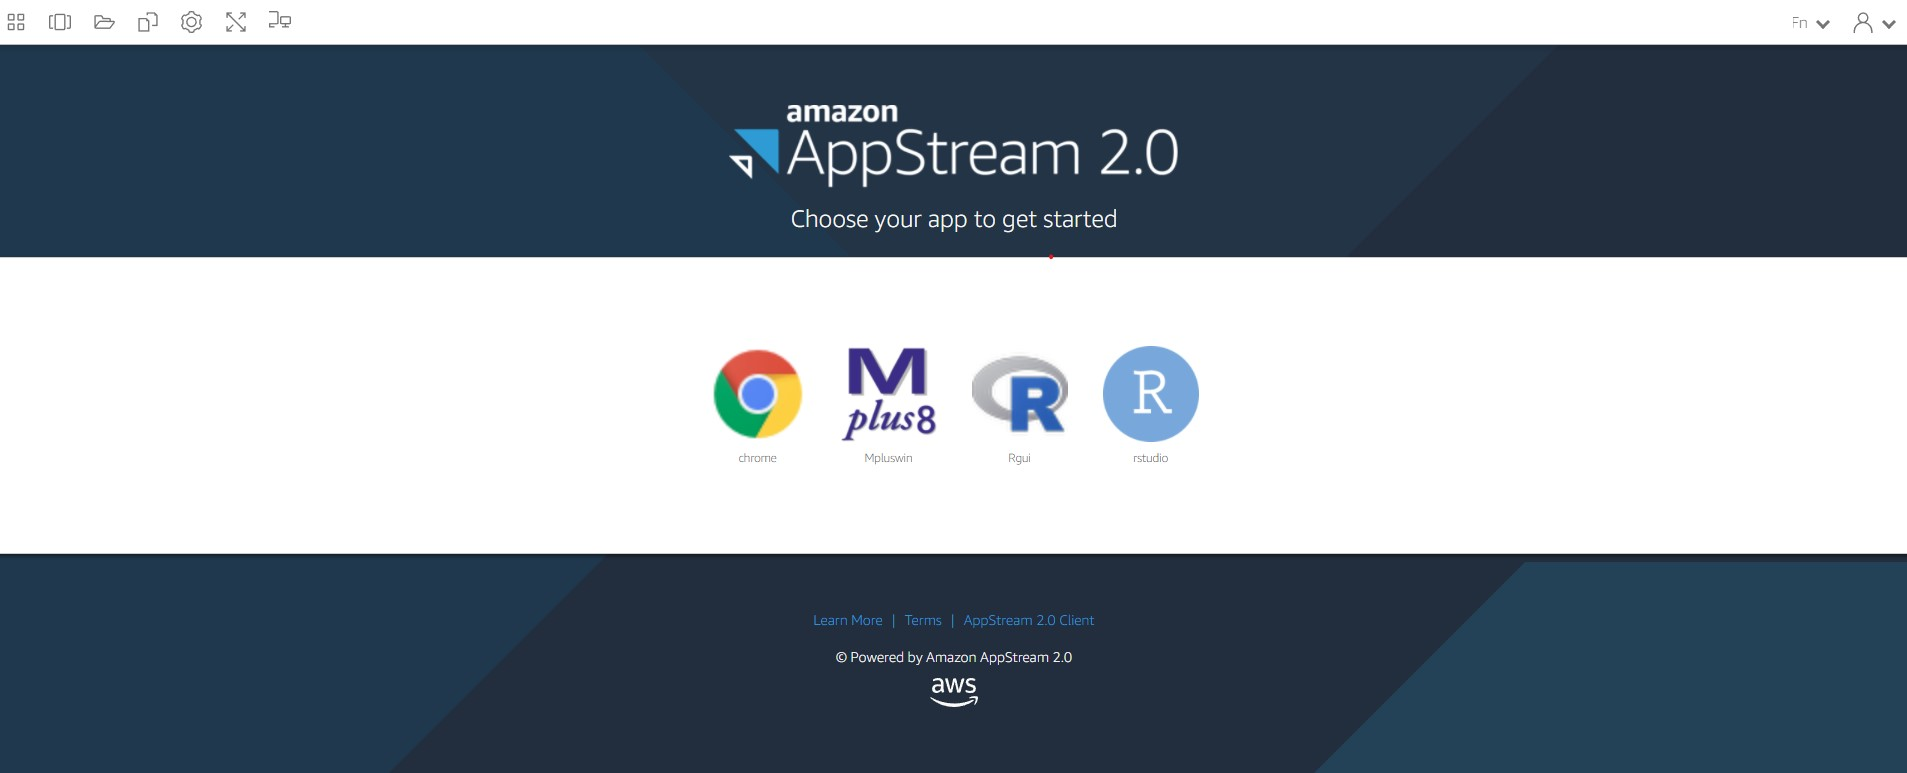
\includegraphics{appstream.jpg}

Follow
\href{https://docs.google.com/document/d/1ligSL9zj7lZIK6VDhF1dLScArrufTd6vLFgcOm05M-4/edit?usp=sharing}{these}
steps to get access to Mplus and RStudio (\emph{Note}: These steps are
not necessary if you already own Mplus). When you get access to the
AppStream space, it takes about two minutes to begin the session. It
would be a good idea to get it open before labs start that way you're
not behind.

\hypertarget{step-2-open-mplus-in-appstream}{%
\subsubsection{Step 2: Open Mplus in
AppStream}\label{step-2-open-mplus-in-appstream}}

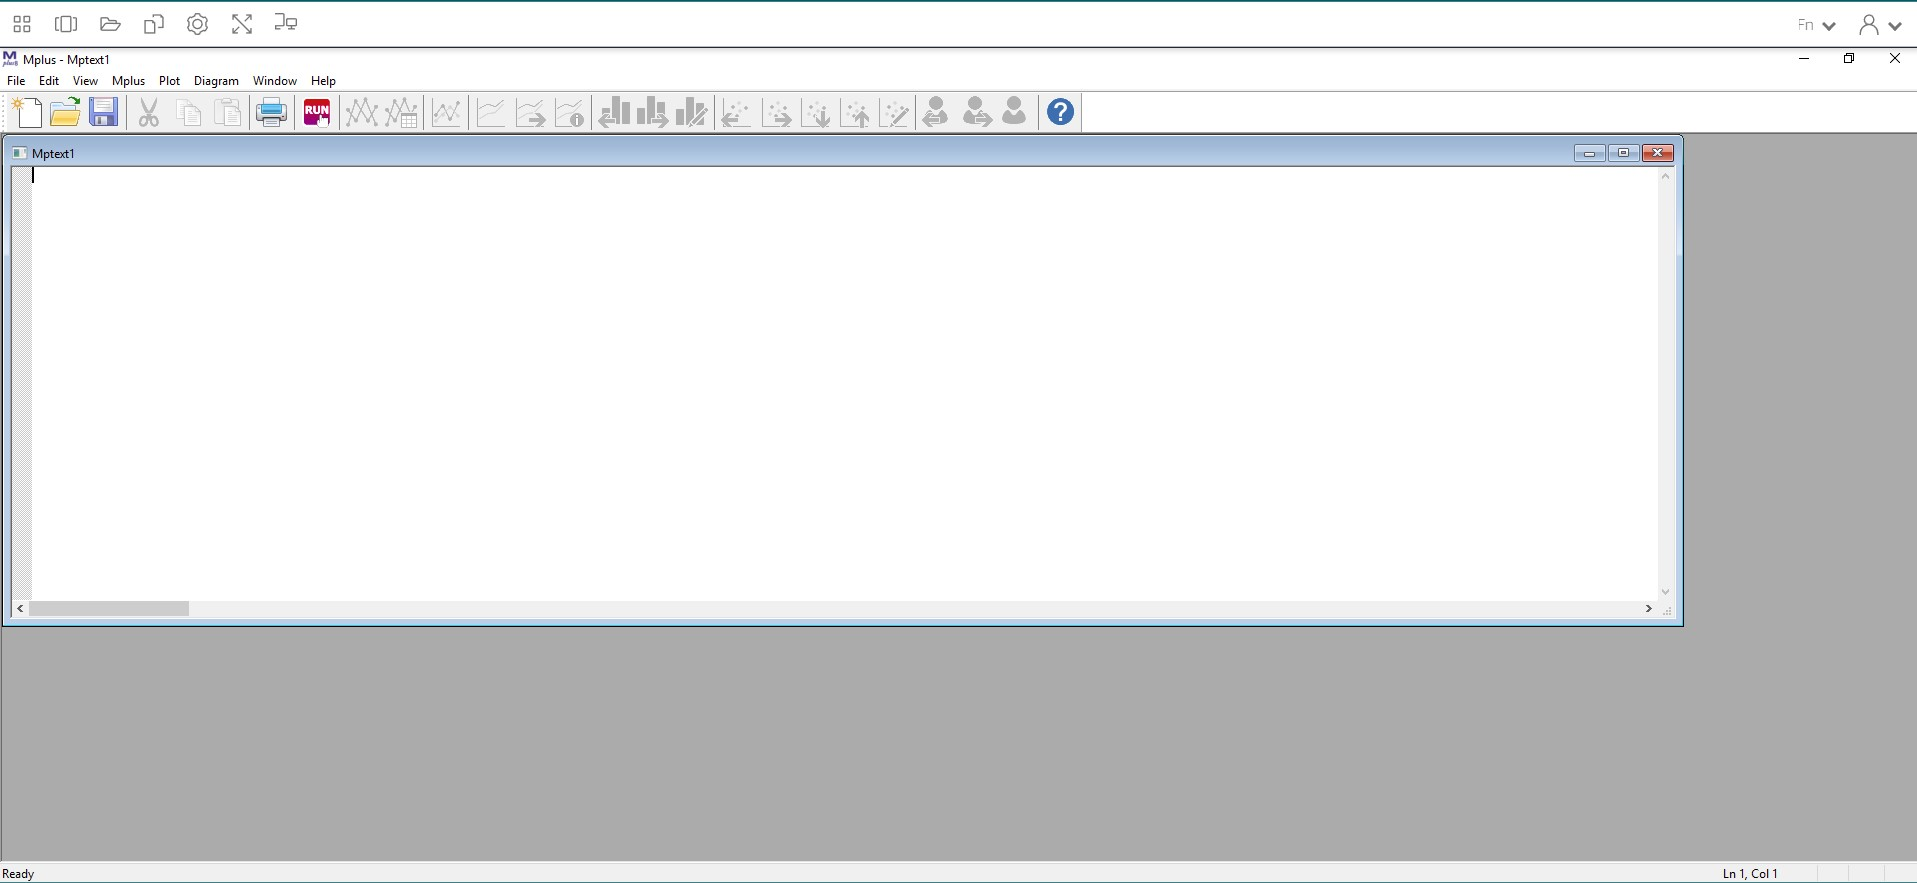
\includegraphics{mplus.jpg}

This is the Mplus interface. Even though we will NOT be working directly
in Mplus for the rest of the quarter, it is good to get an idea of how
Mplus works.

\hypertarget{step-3-link-your-google-drive-to-appstream}{%
\subsubsection{Step 3: Link your Google Drive to
AppStream}\label{step-3-link-your-google-drive-to-appstream}}

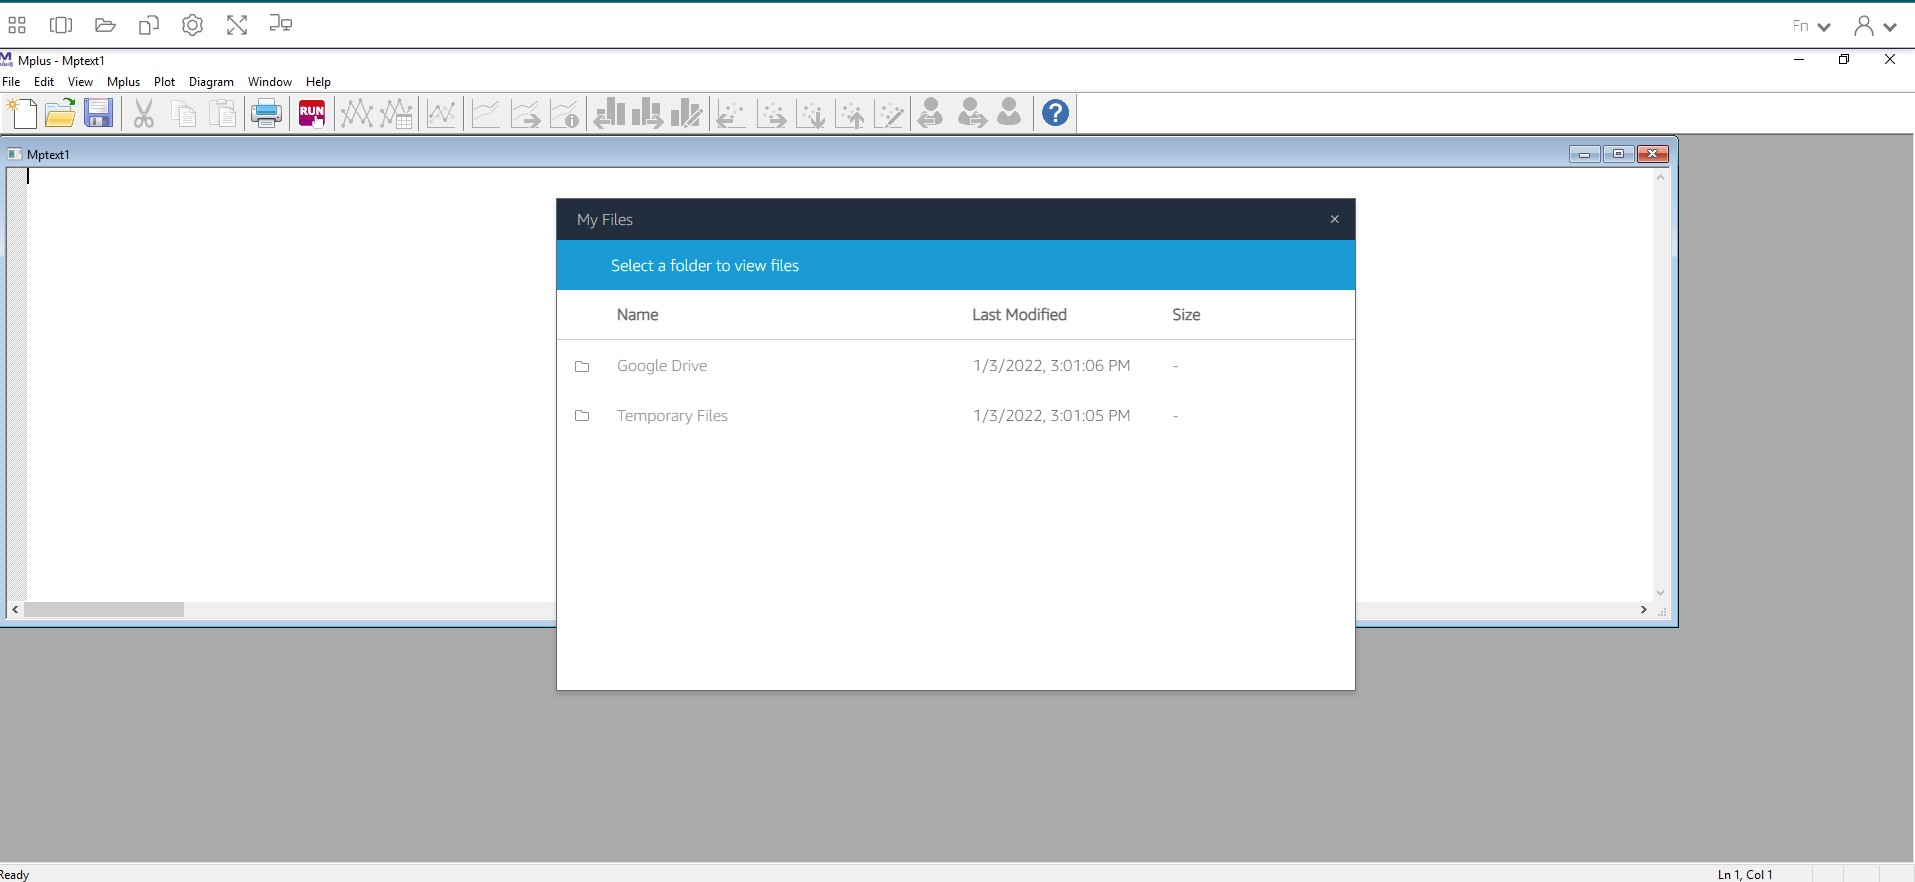
\includegraphics{gd.jpg}

AppStream uses GoogleDrive to access and save all your files that you
work with. It is \textbf{important} to save your files before you close
AppStream as there is no cloud storage. Everything is stored locally
during your session, but upon closing AppStream, your data is cleared.

\hypertarget{step-4-create-a-google-drive-folder-for-this-class-and-import-lab-material}{%
\subsubsection{Step 4: Create a Google Drive folder for this class and
import lab
material}\label{step-4-create-a-google-drive-folder-for-this-class-and-import-lab-material}}

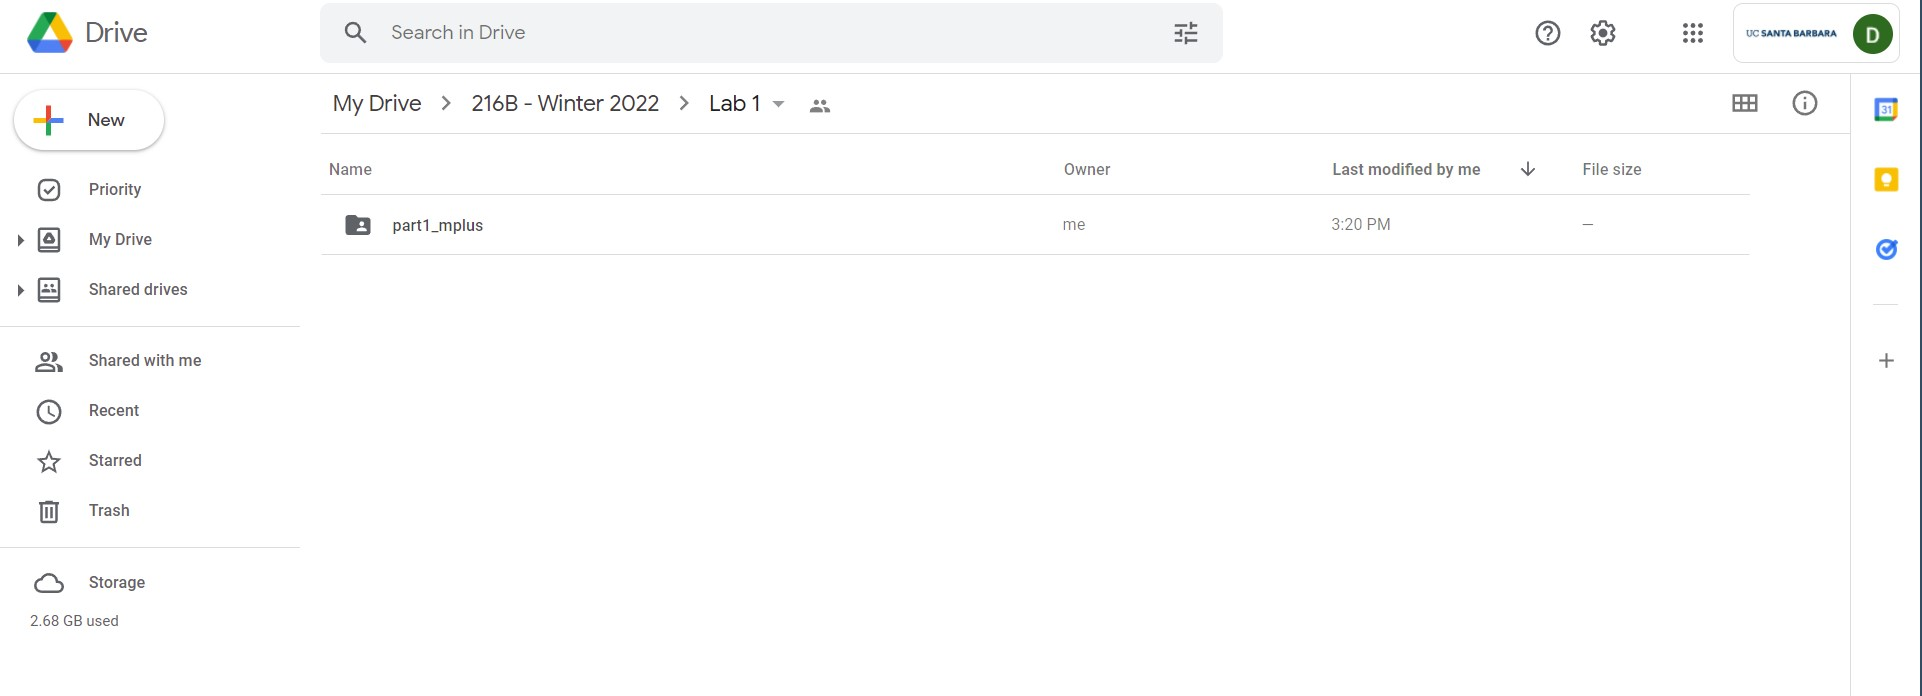
\includegraphics{import.jpg}

Open up a new browser (not in AppStream) and log in to your Google
Drive. Create a new folder for this class so we can start importing and
save into your Google Drive. Go to GauchoSpace and download the lab
materials for this class and import it into this new folder you created.
\emph{Note:} As we go forward with this lab, the location of this folder
will change, just a heads up.

\hypertarget{step-5-import-syntax-into-mplus-from-google-drive}{%
\subsubsection{Step 5: Import syntax into Mplus from Google
Drive}\label{step-5-import-syntax-into-mplus-from-google-drive}}

\includegraphics{inp.gif}

All syntax or input files for Mplus are a \emph{.inp}~file. You may also
create a new \emph{.inp}~file directly in Mplus and populate the syntax
there. For now, we can use one that is already complete.

\begin{itemize}
\item
  Basic skeleton of an Mplus \emph{.inp}~syntax

  \begin{itemize}
  \item
    \textbf{TITLE:} title of our document
  \item
    \textbf{DATA:} data file (must be in the same folder as the
    \emph{.inp})
  \item
    \textbf{VARIABLE:}

    \begin{itemize}
    \item
      \textbf{NAMES =} names of each variable in order of each column
    \item
      \textbf{MISSING} = what the missing data is labeled as
    \item
      \textbf{USEVAR =} names of the variable actually being used in the
      analysis
    \end{itemize}
  \item
    \textbf{ANALYSIS:}

    \begin{itemize}
    \tightlist
    \item
      \textbf{TYPE =} this section is what will change constantly based
      on your model. For now, we are running ``type = basic'' which will
      provide us descriptive statistics of our variables.
    \end{itemize}
  \end{itemize}
\end{itemize}

\textbf{NOTE:} Please view the data file that is provided in this lab
(basic\_Lab1\_DEMO.dat). Mplus works with .dat files to run analyses.
The dataset must also be formatted in certain way in order for Mplus to
read it. Please see ``Mplus Basics'' on GauchoSpace under Mplus
Resources for more information. There is also a codebook that provides
some information on the items on Gauchospace (``Lab 1 Codebook'').

\hypertarget{step-6-click-run}{%
\subsubsection{Step 6: Click Run}\label{step-6-click-run}}

\includegraphics{out.gif}

This will run our ``type=basic'' analysis which will provide us a
\emph{.out} file that contains variables descriptive statistics of our
variables. AppStream will save this \emph{.out}~file in your current
GoogleDrive folder. All \emph{.out} and \emph{.inp} files can be open as
a text file if you want to access them off AppStream/Mplus.

\begin{center}\rule{0.5\linewidth}{0.5pt}\end{center}

\hypertarget{part-2-introduction-to-rstudio}{%
\subsection{\texorpdfstring{\underline{PART 2}: Introduction to
RStudio}{PART 2: Introduction to RStudio}}\label{part-2-introduction-to-rstudio}}

Now, we will be obtaining the same \emph{.out} file that we produced
above using RStudio (and never having to open Mplus!). This is done
using the
\href{chrome-extension://efaidnbmnnnibpcajpcglclefindmkaj/viewer.html?pdfurl=https\%3A\%2F\%2Fcran.r-project.org\%2Fweb\%2Fpackages\%2FMplusAutomation\%2FMplusAutomation.pdf\&clen=322228\&chunk=true}{\texttt{MplusAutomation}}
package (Hallquist \& WIley, 2018). This R package communicates with
Mplus to replicate the process we went through above using Rstudio and R
language. While this course expects you to have some R knowledge, I will
go through some basics here. Please see ``R-Studio Basics'' on
GauchoSpace under R Resources for R tips.

\hypertarget{what-is-mplusautomation-why-should-we-use-it}{%
\subsubsection{\texorpdfstring{WHAT is \texttt{MplusAutomation} \& WHY
should we use
it?}{WHAT is MplusAutomation \& WHY should we use it?}}\label{what-is-mplusautomation-why-should-we-use-it}}

\textbf{WHAT?}

\begin{itemize}
\tightlist
\item
  \texttt{MplusAutomation} is an \texttt{R} package
\item
  It ``wraps around'' the \texttt{Mplus} program
\item
  Requires both \texttt{R} \& \texttt{Mplus} software
\item
  Requires learning some basics of 2 programming languages
\item
  Car metaphor: R/Rstudio is the \emph{steering wheel or dashboard} \&
  Mplus is the \emph{engine}
\end{itemize}

\textbf{WHY?}

\begin{itemize}
\tightlist
\item
  As a data analyst using Mplus to analyze projects that often span
  multiple years I realized a need for clearly organized work procedures
  in which every research decision can be documented in a single place.
\item
  The motivation for using this method is to increase reproducibility,
  organization, efficiency, and transparency
\end{itemize}

\textbf{HOW?}

\begin{itemize}
\tightlist
\item
  We will interface entirely within R-Studio.
\item
  The code presented will be very repetitive by design. Creating a
  consistent routine is key!
\end{itemize}

\hypertarget{step-1-open-rstudio-in-appstream}{%
\subsubsection{Step 1: Open RStudio in
AppStream}\label{step-1-open-rstudio-in-appstream}}

\includegraphics{rstudio.gif}

Open R studio within AppStream. You don't need to close Mplus.
\textbf{IMPORTANT}: Because we are using a package that communicates
with Mplus, we \emph{must} use the AppStream interface to run Rstudio
(unless you already have Mplus available on your personal computer).

\hypertarget{step-2-create-a-new-r-project}{%
\subsubsection{Step 2: Create a new
R-project}\label{step-2-create-a-new-r-project}}

\includegraphics{rproject.gif}

R-projects help us organize our folders , filepaths, and scripts. To
create a new R project:

\begin{itemize}
\tightlist
\item
  File --\textgreater{} New Project\ldots{}
\end{itemize}

Click ``New Directory'' --\textgreater{} New Project --\textgreater{}
Name your project (Perhaps ``lab1'')

Before you click ``Create Project,'' save your project under ``My
Drive''. \textbf{THIS IS IMPORTANT.} If your file path is too long
(longer than 90 characters), then Mplus cuts off the filepath and will
not run your syntax. Move all your Lab 1 Materials into this new project
folder you have created.

\hypertarget{step-3-create-an-r-markdown-document}{%
\subsubsection{Step 3: Create an R-markdown
document}\label{step-3-create-an-r-markdown-document}}

\includegraphics{rmarkdown.gif}

An R-markdown file provides an authoring framework for data science that
allows us to organize our reports using texts and code chunks. This
document you are reading was made using R-markdown! Lets create an
R-markdown and write script to run a ``type=basic'' analysis using the R
package, \texttt{MplusAutomation}.

To create an R-markdown:

\begin{itemize}
\tightlist
\item
  File --\textgreater{} New File --\textgreater{} R Markdown\ldots{}
\end{itemize}

\textbf{Note}: AppStream may ask you to update R markdown. Click
``Yes.''

In the window that pops up, give the R-markdown a title such as
``\textbf{Lab 1 - Introduction to RStudio.}'' Click ``OK.'' You should
see a new markdown with some example text and code chunks. We want a
clean document to start off with so delete everything from line 10 down.
Go ahead and save this document to your Google Drive folder.

\hypertarget{step-4-load-packages}{%
\subsubsection{Step 4: Load packages}\label{step-4-load-packages}}

Your first code chunk in any given markdown should be the packages you
will be using. To insert a code chunk, etiher use the keyboard shortcut
ctrl + alt + i or Code --\textgreater{} Insert Chunk or click the green
box with the letter C on it. There are a few packages we want our
markdown to read in:

\begin{Shaded}
\begin{Highlighting}[]
\FunctionTok{library}\NormalTok{(MplusAutomation)}
\FunctionTok{library}\NormalTok{(tidyverse) }\CommentTok{\#collection of R packages designed for data science}
\FunctionTok{library}\NormalTok{(here) }\CommentTok{\#helps with filepaths}
\FunctionTok{library}\NormalTok{(haven) }\CommentTok{\# read\_sav()}
\FunctionTok{library}\NormalTok{(psych) }\CommentTok{\# describe()}
\FunctionTok{library}\NormalTok{(ggpubr) }\CommentTok{\# ggdensity() and ggqqplot()}
\FunctionTok{library}\NormalTok{(corrplot) }\CommentTok{\# corrplot()}
\end{Highlighting}
\end{Shaded}

As a reminder, if a function does not work and you receive an error like
this: \texttt{could\ not\ find\ function\ "random\_function"}; or if you
try to load a package and you receive an error like this:
\texttt{there\ is\ no\ package\ called\ \textasciigrave{}random\_package\textasciigrave{}}
, then you will need to install the package using
\texttt{install.packages("random\_package")} in the console (the
bottom-left window in R studio). Once you have installed the package you
will \emph{never} need to install it again, however you must
\emph{always} load in the packages at the beginning of your R markdown
using \texttt{library(random\_package)}, as shown in this document.

\textbf{NOTE}: With AppStream, we pre-installed most packages. However,
there may be some we missed and those may need to be installed with each
session. If you are using R studio on your personal computer, then once
it is installed, it doesn't need to be installed again.

\hypertarget{step-5-read-in-data-set}{%
\subsubsection{Step 5: Read in data set}\label{step-5-read-in-data-set}}

Recall that our data set that we used earlier is a \emph{.dat}~file with
no variable names. Remember that this is a data set specifically
designed for Mplus. Let grab the original one (an SPSS file) in the
\texttt{data} folder within the \texttt{part2\_rstudio} folder.

\begin{Shaded}
\begin{Highlighting}[]
\NormalTok{data }\OtherTok{\textless{}{-}} \FunctionTok{read\_sav}\NormalTok{(}\FunctionTok{here}\NormalTok{(}\StringTok{"part2\_rstudio"}\NormalTok{, }\StringTok{"data"}\NormalTok{, }\StringTok{"explore\_lab\_data.sav"}\NormalTok{))}

\CommentTok{\# Ways to view data in R:}
\CommentTok{\# 1. click on the data in your Global Environment (upper right pane) or use...}
\FunctionTok{View}\NormalTok{(data)}
\CommentTok{\# 2. summary() gives basic summary statistics \& shows number of NA values}
\CommentTok{\# *great for checking that data has been read in correctly*}
\FunctionTok{summary}\NormalTok{(data)}
\end{Highlighting}
\end{Shaded}

\begin{verbatim}
##      item1            item2            item3            item4       
##  Min.   : 1.000   Min.   : 1.000   Min.   : 1.000   Min.   : 1.000  
##  1st Qu.: 2.000   1st Qu.: 2.000   1st Qu.: 2.000   1st Qu.: 2.000  
##  Median : 4.000   Median : 5.000   Median : 5.000   Median : 5.000  
##  Mean   : 4.508   Mean   : 4.856   Mean   : 4.706   Mean   : 4.815  
##  3rd Qu.: 6.000   3rd Qu.: 7.000   3rd Qu.: 7.000   3rd Qu.: 7.000  
##  Max.   :10.000   Max.   :10.000   Max.   :10.000   Max.   :10.000  
##                   NA's   :1                                         
##      item5            item6           item7            item8       
##  Min.   : 1.000   Min.   : 1.00   Min.   : 1.000   Min.   : 1.000  
##  1st Qu.: 2.000   1st Qu.: 2.00   1st Qu.: 1.000   1st Qu.: 1.000  
##  Median : 3.000   Median : 5.00   Median : 3.000   Median : 3.000  
##  Mean   : 4.169   Mean   : 4.72   Mean   : 3.689   Mean   : 3.915  
##  3rd Qu.: 6.000   3rd Qu.: 7.00   3rd Qu.: 5.000   3rd Qu.: 6.000  
##  Max.   :25.000   Max.   :10.00   Max.   :10.000   Max.   :10.000  
##  NA's   :1        NA's   :1                        NA's   :1       
##      item9            female      
##  Min.   : 1.000   Min.   :0.0000  
##  1st Qu.: 4.000   1st Qu.:0.0000  
##  Median : 6.000   Median :1.0000  
##  Mean   : 5.857   Mean   :0.6807  
##  3rd Qu.: 8.000   3rd Qu.:1.0000  
##  Max.   :10.000   Max.   :1.0000  
## 
\end{verbatim}

\begin{Shaded}
\begin{Highlighting}[]
\CommentTok{\# 3. names() provides a list of column names. Very useful if you don\textquotesingle{}t have them memorized!}
\FunctionTok{names}\NormalTok{(data)}
\end{Highlighting}
\end{Shaded}

\begin{verbatim}
##  [1] "item1"  "item2"  "item3"  "item4"  "item5"  "item6"  "item7"  "item8" 
##  [9] "item9"  "female"
\end{verbatim}

\begin{Shaded}
\begin{Highlighting}[]
\CommentTok{\# 4. head() prints the top x rows of the dataframe}
\FunctionTok{head}\NormalTok{(data)}
\end{Highlighting}
\end{Shaded}

\begin{verbatim}
## # A tibble: 6 x 10
##   item1 item2 item3 item4 item5 item6 item7 item8 item9     female
##   <dbl> <dbl> <dbl> <dbl> <dbl> <dbl> <dbl> <dbl> <dbl>  <dbl+lbl>
## 1     2     1     1     1     1     1     1     1     1 1 [female]
## 2     2     2     1     1     1     2     1     1     1 1 [female]
## 3     3     2     3     3     1     2     1     1     1 1 [female]
## 4     1     2     1     1     1     4     1     1     1 0 [male]  
## 5     2     1     1     3     1     1     2     1     1 1 [female]
## 6     3     1     2     1     3     2     2     2     1 1 [female]
\end{verbatim}

You can also look at the dataframe with labels and response scale
meta-data:

\begin{Shaded}
\begin{Highlighting}[]
\NormalTok{sjPlot}\SpecialCharTok{::}\FunctionTok{view\_df}\NormalTok{(data)}
\end{Highlighting}
\end{Shaded}

Data frame: data

ID

Name

Label

Values

Value Labels

1

item1

range: 1.0-10.0

2

item2

range: 1-10

3

item3

range: 1-10

4

item4

range: 1-10

5

item5

range: 1-25

6

item6

range: 1-10

7

item7

range: 1-10

8

item8

range: 1-10

9

item9

range: 1-10

10

female

Student gender

01

malefemale

This SPSS dataset gives us more information than the \emph{.dat}~one. We
are able to see the variable names, and descriptions.

\textbf{Convert from \emph{.sav} to \emph{.csv}}

It's a good idea to convert \emph{.sav} files to \emph{.csv}. Here is
how to convert the \textbf{\emph{.sav}} \textbf{to \emph{.csv}}:

\begin{Shaded}
\begin{Highlighting}[]
\CommentTok{\# write\_csv saves a .csv version of your dataset to your working directory.}
\CommentTok{\# Enter the name of the object that contains your data set (in this case, "exp\_lab1\_data.csv"), then enter the name you want to save your dataset as. We can call it the same thing: "screen1.csv"}
\FunctionTok{write\_csv}\NormalTok{(data, }\FunctionTok{here}\NormalTok{(}\StringTok{"part2\_rstudio"}\NormalTok{, }\StringTok{"data"}\NormalTok{, }\StringTok{"exp\_lab1\_data.csv"}\NormalTok{))}

\CommentTok{\# read the unlabeled data back into R}
\NormalTok{data\_csv }\OtherTok{\textless{}{-}} \FunctionTok{read\_csv}\NormalTok{(}\FunctionTok{here}\NormalTok{(}\StringTok{"part2\_rstudio"}\NormalTok{, }\StringTok{"data"}\NormalTok{, }\StringTok{"exp\_lab1\_data.csv"}\NormalTok{))}
\end{Highlighting}
\end{Shaded}

\textbf{Optional: Convert from \emph{.csv} to Mplus \emph{.dat} file}

Say you want an Mplus .dat file and don't want to go through the hassle
of deleting rows and manual conversion to \emph{.dat}. You can use the
\texttt{prepareMplusData()} function to convert from \emph{.csv} to
\emph{.dat}.

\begin{Shaded}
\begin{Highlighting}[]
\FunctionTok{prepareMplusData}\NormalTok{(data\_csv, }\FunctionTok{here}\NormalTok{(}\StringTok{"part2\_rstudio"}\NormalTok{, }\StringTok{"data"}\NormalTok{, }\StringTok{"exp\_lab1\_data.dat"}\NormalTok{))}
\end{Highlighting}
\end{Shaded}

\begin{verbatim}
## TITLE: Your title goes here
## DATA: FILE = "C:/Users/Dina Arch/Box/TA - ED 216B/Labs/part2_rstudio/data/exp_lab1_data.dat";
## VARIABLE: 
## NAMES = item1 item2 item3 item4 item5 item6 item7 item8 item9 female; 
## MISSING=.;
\end{verbatim}

\hypertarget{step-6-using-mplusautomation}{%
\subsubsection{\texorpdfstring{Step 6: Using
\texttt{MplusAutomation}}{Step 6: Using MplusAutomation}}\label{step-6-using-mplusautomation}}

To run a basic model using \texttt{MplusAutomation} we used the
\texttt{mplusObject()} function and the \texttt{mplusModeler()}
function.

\textbf{What does the} \texttt{mplusObject()} \textbf{function do?}

1. It generates an Mplus input file (does not need full variable name
list, its automated for you!) 2. It generates a datafile specific to
each model 3. It runs or estimates the model (hopefully) producing the
correct output. Always check!

\textbf{What does the} \texttt{mplusModeler()} \textbf{function do?}

\begin{enumerate}
\def\labelenumi{\arabic{enumi}.}
\tightlist
\item
  Creates, runs, and reads Mplus models created using
  \texttt{mplusObject()}
\item
  You can specify where you want the \emph{.out}~file saved
\item
  \texttt{check=TRUE} checks for missing semicolons, \texttt{run=TRUE}
  runs the model, \texttt{hashfilename=FALSE} does not add a hash of the
  raw data to the datafile name.
\end{enumerate}

\begin{Shaded}
\begin{Highlighting}[]
\NormalTok{m\_basic  }\OtherTok{\textless{}{-}} \FunctionTok{mplusObject}\NormalTok{(}
  
  \AttributeTok{TITLE =} \StringTok{"PRACTICE 01 {-} Explore TYPE = BASIC;"}\NormalTok{,}
  
  \AttributeTok{VARIABLE =} 
 \StringTok{"usevar= item1 item2 item3 item4 item5 item6 item7 item8 item9 female;"}\NormalTok{,}
  
  \AttributeTok{ANALYSIS =} 
 \StringTok{"type = basic; "}\NormalTok{,}
 
  \AttributeTok{usevariables =} \FunctionTok{colnames}\NormalTok{(data\_csv), }
  \AttributeTok{rdata =}\NormalTok{ data\_csv)}

\NormalTok{m\_basic\_fit }\OtherTok{\textless{}{-}} \FunctionTok{mplusModeler}\NormalTok{(m\_basic, }
               \AttributeTok{dataout=}\FunctionTok{here}\NormalTok{(}\StringTok{"part2\_rstudio"}\NormalTok{, }\StringTok{"basic.dat"}\NormalTok{),}
               \AttributeTok{modelout=}\FunctionTok{here}\NormalTok{(}\StringTok{"part2\_rstudio"}\NormalTok{, }\StringTok{"basic.inp"}\NormalTok{),}
               \AttributeTok{check=}\ConstantTok{TRUE}\NormalTok{, }\AttributeTok{run =} \ConstantTok{TRUE}\NormalTok{, }\AttributeTok{hashfilename =} \ConstantTok{FALSE}\NormalTok{)}
\end{Highlighting}
\end{Shaded}

\textbf{NOTE}: You don't need to specify \texttt{MISSING} here since it
automatically detects the missing value from the data set. You also
don't need \texttt{NAMES} as it detects the names from the data set.

\textbf{Optional: Subsetting observations}

You can use Mplus syntax to explore descriptives for observations
reported as ``female.''

Add line of syntax: \texttt{useobs\ =\ female\ ==\ 1;}

\begin{Shaded}
\begin{Highlighting}[]
\NormalTok{fem\_basic  }\OtherTok{\textless{}{-}} \FunctionTok{mplusObject}\NormalTok{(}
  
  \AttributeTok{TITLE =} \StringTok{"PRACTICE 02 {-} Explore female observations only;"}\NormalTok{, }
  
  \AttributeTok{VARIABLE =} 
  \StringTok{"usevar = item1 item2 item3 item4 item5 item6 item7 item8 item9;}
\StringTok{  useobs = female == 1; !include observations that report female in analysis"}\NormalTok{,}
  
  \AttributeTok{ANALYSIS =} 
    \StringTok{"type = basic;"}\NormalTok{,}
 
  \AttributeTok{usevariables =} \FunctionTok{colnames}\NormalTok{(data\_csv), }
  \AttributeTok{rdata =}\NormalTok{ data\_csv)}

\NormalTok{fem\_basic\_fit }\OtherTok{\textless{}{-}} \FunctionTok{mplusModeler}\NormalTok{(m\_basic, }
               \AttributeTok{dataout=}\FunctionTok{here}\NormalTok{(}\StringTok{"part2\_rstudio"}\NormalTok{, }\StringTok{"fem\_basic.dat"}\NormalTok{),}
               \AttributeTok{modelout=}\FunctionTok{here}\NormalTok{(}\StringTok{"part2\_rstudio"}\NormalTok{, }\StringTok{"fem\_basic.inp"}\NormalTok{),}
               \AttributeTok{check=}\ConstantTok{TRUE}\NormalTok{, }\AttributeTok{run =} \ConstantTok{TRUE}\NormalTok{, }\AttributeTok{hashfilename =} \ConstantTok{FALSE}\NormalTok{)}
\end{Highlighting}
\end{Shaded}

\begin{center}\rule{0.5\linewidth}{0.5pt}\end{center}

\hypertarget{part-3-data-cleaning-screening}{%
\subsection{\texorpdfstring{\underline{PART 3}: Data Cleaning \&
Screening}{PART 3: Data Cleaning \& Screening}}\label{part-3-data-cleaning-screening}}

It's important to explore your variables before running a factor
analysis. First, lets rename our variables to something more meaningful
using \texttt{rename()}. As a reminder, use the pipe operator
\texttt{\%\textgreater{}\%} to create a sequence of functions, you can
use the shortcut crt + shift + m:

\begin{Shaded}
\begin{Highlighting}[]
\NormalTok{new\_names }\OtherTok{\textless{}{-}}\NormalTok{ data\_csv }\SpecialCharTok{\%\textgreater{}\%}
  \FunctionTok{rename}\NormalTok{(}\AttributeTok{school\_motiv1 =}\NormalTok{ item1,}
         \AttributeTok{school\_motiv2 =}\NormalTok{ item2,}
         \AttributeTok{school\_motiv3 =}\NormalTok{ item3,}
         \AttributeTok{school\_comp1 =}\NormalTok{ item4,}
         \AttributeTok{school\_comp2 =}\NormalTok{ item5,}
         \AttributeTok{school\_comp3 =}\NormalTok{ item6,}
         \AttributeTok{school\_belif1 =}\NormalTok{ item7,}
         \AttributeTok{school\_belif2 =}\NormalTok{ item8,}
         \AttributeTok{school\_belif3 =}\NormalTok{ item9)}
\end{Highlighting}
\end{Shaded}

\hypertarget{descriptive-statistics}{%
\subsubsection{Descriptive Statistics}\label{descriptive-statistics}}

Let's look at descriptive statistics for each variable using
\texttt{summary()}:

\begin{Shaded}
\begin{Highlighting}[]
\NormalTok{new\_names }\SpecialCharTok{\%\textgreater{}\%} 
  \FunctionTok{summary}\NormalTok{() }
\end{Highlighting}
\end{Shaded}

\begin{verbatim}
##  school_motiv1    school_motiv2    school_motiv3     school_comp1   
##  Min.   : 1.000   Min.   : 1.000   Min.   : 1.000   Min.   : 1.000  
##  1st Qu.: 2.000   1st Qu.: 2.000   1st Qu.: 2.000   1st Qu.: 2.000  
##  Median : 4.000   Median : 5.000   Median : 5.000   Median : 5.000  
##  Mean   : 4.508   Mean   : 4.856   Mean   : 4.706   Mean   : 4.815  
##  3rd Qu.: 6.000   3rd Qu.: 7.000   3rd Qu.: 7.000   3rd Qu.: 7.000  
##  Max.   :10.000   Max.   :10.000   Max.   :10.000   Max.   :10.000  
##                   NA's   :1                                         
##   school_comp2     school_comp3   school_belif1    school_belif2   
##  Min.   : 1.000   Min.   : 1.00   Min.   : 1.000   Min.   : 1.000  
##  1st Qu.: 2.000   1st Qu.: 2.00   1st Qu.: 1.000   1st Qu.: 1.000  
##  Median : 3.000   Median : 5.00   Median : 3.000   Median : 3.000  
##  Mean   : 4.169   Mean   : 4.72   Mean   : 3.689   Mean   : 3.915  
##  3rd Qu.: 6.000   3rd Qu.: 7.00   3rd Qu.: 5.000   3rd Qu.: 6.000  
##  Max.   :25.000   Max.   :10.00   Max.   :10.000   Max.   :10.000  
##  NA's   :1        NA's   :1                        NA's   :1       
##  school_belif3        female      
##  Min.   : 1.000   Min.   :0.0000  
##  1st Qu.: 4.000   1st Qu.:0.0000  
##  Median : 6.000   Median :1.0000  
##  Mean   : 5.857   Mean   :0.6807  
##  3rd Qu.: 8.000   3rd Qu.:1.0000  
##  Max.   :10.000   Max.   :1.0000  
## 
\end{verbatim}

Alternatively, we can use the \texttt{psych::describe()} function to
give more information:

\begin{Shaded}
\begin{Highlighting}[]
\NormalTok{new\_names }\SpecialCharTok{\%\textgreater{}\%} 
  \FunctionTok{describe}\NormalTok{()}
\end{Highlighting}
\end{Shaded}

\begin{verbatim}
##               vars   n mean   sd median trimmed  mad min max range  skew
## school_motiv1    1 119 4.51 2.64      4    4.36 2.97   1  10     9  0.31
## school_motiv2    2 118 4.86 2.72      5    4.76 2.97   1  10     9  0.14
## school_motiv3    3 119 4.71 2.74      5    4.56 2.97   1  10     9  0.31
## school_comp1     4 119 4.82 2.80      5    4.71 2.97   1  10     9  0.18
## school_comp2     5 118 4.17 3.31      3    3.79 2.97   1  25    24  2.30
## school_comp3     6 118 4.72 2.69      5    4.66 4.45   1  10     9  0.14
## school_belif1    7 119 3.69 2.80      3    3.36 2.97   1  10     9  0.87
## school_belif2    8 118 3.92 2.85      3    3.65 2.97   1  10     9  0.62
## school_belif3    9 119 5.86 2.68      6    5.90 2.97   1  10     9 -0.19
## female          10 119 0.68 0.47      1    0.72 0.00   0   1     1 -0.77
##               kurtosis   se
## school_motiv1    -0.91 0.24
## school_motiv2    -1.13 0.25
## school_motiv3    -1.02 0.25
## school_comp1     -1.22 0.26
## school_comp2     11.15 0.30
## school_comp3     -1.29 0.25
## school_belif1    -0.58 0.26
## school_belif2    -0.96 0.26
## school_belif3    -1.08 0.25
## female           -1.43 0.04
\end{verbatim}

What if we want to look at a subset of the data? For example, what if we
want to see those who identify as female? We can use
\texttt{tidyverse::filter()} to subset the data using certain criteria.

\begin{Shaded}
\begin{Highlighting}[]
\NormalTok{new\_names }\SpecialCharTok{\%\textgreater{}\%} 
  \FunctionTok{filter}\NormalTok{(female }\SpecialCharTok{==} \DecValTok{1}\NormalTok{) }\SpecialCharTok{\%\textgreater{}\%} 
  \FunctionTok{describe}\NormalTok{()}
\end{Highlighting}
\end{Shaded}

\begin{verbatim}
##               vars  n mean   sd median trimmed  mad min max range  skew
## school_motiv1    1 81 4.61 2.60    4.5    4.48 3.71   1  10     9  0.29
## school_motiv2    2 80 4.92 2.62    5.0    4.88 2.97   1  10     9  0.06
## school_motiv3    3 81 4.85 2.80    5.0    4.74 2.97   1  10     9  0.21
## school_comp1     4 81 4.93 2.75    5.0    4.86 2.97   1  10     9  0.13
## school_comp2     5 80 4.19 3.49    3.0    3.75 2.97   1  25    24  2.75
## school_comp3     6 80 4.74 2.69    5.0    4.70 4.45   1  10     9  0.06
## school_belif1    7 81 3.77 2.86    3.0    3.42 2.97   1  10     9  0.82
## school_belif2    8 80 3.90 2.90    3.0    3.59 2.97   1  10     9  0.64
## school_belif3    9 81 5.68 2.86    6.0    5.69 2.97   1  10     9 -0.06
## female          10 81 1.00 0.00    1.0    1.00 0.00   1   1     0   NaN
##               kurtosis   se
## school_motiv1    -0.87 0.29
## school_motiv2    -1.07 0.29
## school_motiv3    -1.18 0.31
## school_comp1     -1.24 0.31
## school_comp2     13.33 0.39
## school_comp3     -1.39 0.30
## school_belif1    -0.69 0.32
## school_belif2    -0.97 0.32
## school_belif3    -1.27 0.32
## female             NaN 0.00
\end{verbatim}

\begin{Shaded}
\begin{Highlighting}[]
\CommentTok{\#You can use any operator to filter: \textgreater{}, \textless{}, ==, \textgreater{}=, etc.}
\end{Highlighting}
\end{Shaded}

\hypertarget{missing-values}{%
\subsubsection{Missing Values}\label{missing-values}}

Let's check for missing values. First, how are missing values
identified? They could be \texttt{-999}, \texttt{NA}, or literally
anything else. The simplest way to do this is to look back at the
\texttt{summary()} function. There are four variables with one missing
value.

\begin{Shaded}
\begin{Highlighting}[]
\NormalTok{new\_names }\SpecialCharTok{\%\textgreater{}\%} 
  \FunctionTok{summary}\NormalTok{() }
\end{Highlighting}
\end{Shaded}

\begin{verbatim}
##  school_motiv1    school_motiv2    school_motiv3     school_comp1   
##  Min.   : 1.000   Min.   : 1.000   Min.   : 1.000   Min.   : 1.000  
##  1st Qu.: 2.000   1st Qu.: 2.000   1st Qu.: 2.000   1st Qu.: 2.000  
##  Median : 4.000   Median : 5.000   Median : 5.000   Median : 5.000  
##  Mean   : 4.508   Mean   : 4.856   Mean   : 4.706   Mean   : 4.815  
##  3rd Qu.: 6.000   3rd Qu.: 7.000   3rd Qu.: 7.000   3rd Qu.: 7.000  
##  Max.   :10.000   Max.   :10.000   Max.   :10.000   Max.   :10.000  
##                   NA's   :1                                         
##   school_comp2     school_comp3   school_belif1    school_belif2   
##  Min.   : 1.000   Min.   : 1.00   Min.   : 1.000   Min.   : 1.000  
##  1st Qu.: 2.000   1st Qu.: 2.00   1st Qu.: 1.000   1st Qu.: 1.000  
##  Median : 3.000   Median : 5.00   Median : 3.000   Median : 3.000  
##  Mean   : 4.169   Mean   : 4.72   Mean   : 3.689   Mean   : 3.915  
##  3rd Qu.: 6.000   3rd Qu.: 7.00   3rd Qu.: 5.000   3rd Qu.: 6.000  
##  Max.   :25.000   Max.   :10.00   Max.   :10.000   Max.   :10.000  
##  NA's   :1        NA's   :1                        NA's   :1       
##  school_belif3        female      
##  Min.   : 1.000   Min.   :0.0000  
##  1st Qu.: 4.000   1st Qu.:0.0000  
##  Median : 6.000   Median :1.0000  
##  Mean   : 5.857   Mean   :0.6807  
##  3rd Qu.: 8.000   3rd Qu.:1.0000  
##  Max.   :10.000   Max.   :1.0000  
## 
\end{verbatim}

\begin{Shaded}
\begin{Highlighting}[]
\CommentTok{\# summary(new\_names)}
\end{Highlighting}
\end{Shaded}

\hypertarget{recode-continuous-variable-into-factor}{%
\subsubsection{Recode Continuous Variable into
Factor}\label{recode-continuous-variable-into-factor}}

What if you want to recode a continuous variable into different levels
(e.g., high, medium, and low)? Let's use the variable
\texttt{school\_belief1} as an example. First, let's recall the
descriptives:

\begin{Shaded}
\begin{Highlighting}[]
\NormalTok{new\_names }\SpecialCharTok{\%\textgreater{}\%} 
  \FunctionTok{select}\NormalTok{(school\_belif1) }\SpecialCharTok{\%\textgreater{}\%} 
  \FunctionTok{summary}\NormalTok{() }
\end{Highlighting}
\end{Shaded}

\begin{verbatim}
##  school_belif1   
##  Min.   : 1.000  
##  1st Qu.: 1.000  
##  Median : 3.000  
##  Mean   : 3.689  
##  3rd Qu.: 5.000  
##  Max.   :10.000
\end{verbatim}

Here, we can see that the values range from 1 - 10. Lets recode the
variable to look like this:

\begin{longtable}[]{@{}
  >{\raggedright\arraybackslash}p{(\columnwidth - 2\tabcolsep) * \real{0.43}}
  >{\raggedright\arraybackslash}p{(\columnwidth - 2\tabcolsep) * \real{0.43}}@{}}
\toprule
\endhead
Low & 1 - 3 \\
Medium & 4 - 6 \\
High & 7 - 10 \\
\bottomrule
\end{longtable}

We use \texttt{cut()} to divide continuous variables into intervals:

\begin{Shaded}
\begin{Highlighting}[]
\NormalTok{school\_factor }\OtherTok{\textless{}{-}}\NormalTok{ new\_names }\SpecialCharTok{\%\textgreater{}\%} 
  \FunctionTok{mutate}\NormalTok{(}\AttributeTok{school\_factor =} \FunctionTok{cut}\NormalTok{(school\_belif1,}
                      \AttributeTok{breaks =} \FunctionTok{c}\NormalTok{(}\DecValTok{0}\NormalTok{, }\DecValTok{3}\NormalTok{, }\DecValTok{6}\NormalTok{, }\DecValTok{10}\NormalTok{), }\CommentTok{\#Use 0 at the beginning to ensure that 1 is included in the first break, then break by last number in each section (3, 6, 10) }
                      \AttributeTok{labels =} \FunctionTok{c}\NormalTok{(}\StringTok{"low"}\NormalTok{, }\StringTok{"medium"}\NormalTok{, }\StringTok{"high"}\NormalTok{)))}
\CommentTok{\# View summary}
\NormalTok{school\_factor }\SpecialCharTok{\%\textgreater{}\%} 
  \FunctionTok{select}\NormalTok{(school\_belif1, school\_factor) }\SpecialCharTok{\%\textgreater{}\%} 
  \FunctionTok{summary}\NormalTok{() }
\end{Highlighting}
\end{Shaded}

\begin{verbatim}
##  school_belif1    school_factor
##  Min.   : 1.000   low   :72    
##  1st Qu.: 1.000   medium:21    
##  Median : 3.000   high  :26    
##  Mean   : 3.689                
##  3rd Qu.: 5.000                
##  Max.   :10.000
\end{verbatim}

\hypertarget{normality-and-distributions}{%
\subsubsection{Normality and
Distributions}\label{normality-and-distributions}}

It's important to inspect our data to see if it is normally distributed.
Many analyses are sensitive to violations of normality so in order to
make sure we are confident that our data are normal, there are several
things we can look at: density plots, histograms, QQ plots, box plots,
scatterplots, and the descriptives such as skewness and kurtosis.
Normally, we would want to inspect every variable, but for demonstration
purposes, lets focus on the \texttt{school\_belif1} variable.

\hypertarget{density-plots}{%
\paragraph{Density Plots}\label{density-plots}}

A density plot is a visualization of the data over a continuous
interval. As we can see by this density plot, the variable
\texttt{school\_belif1} is positively skewed.

\begin{Shaded}
\begin{Highlighting}[]
\FunctionTok{ggdensity}\NormalTok{(new\_names}\SpecialCharTok{$}\NormalTok{school\_belif1, }\AttributeTok{fill =} \StringTok{"lightgray"}\NormalTok{)}
\end{Highlighting}
\end{Shaded}

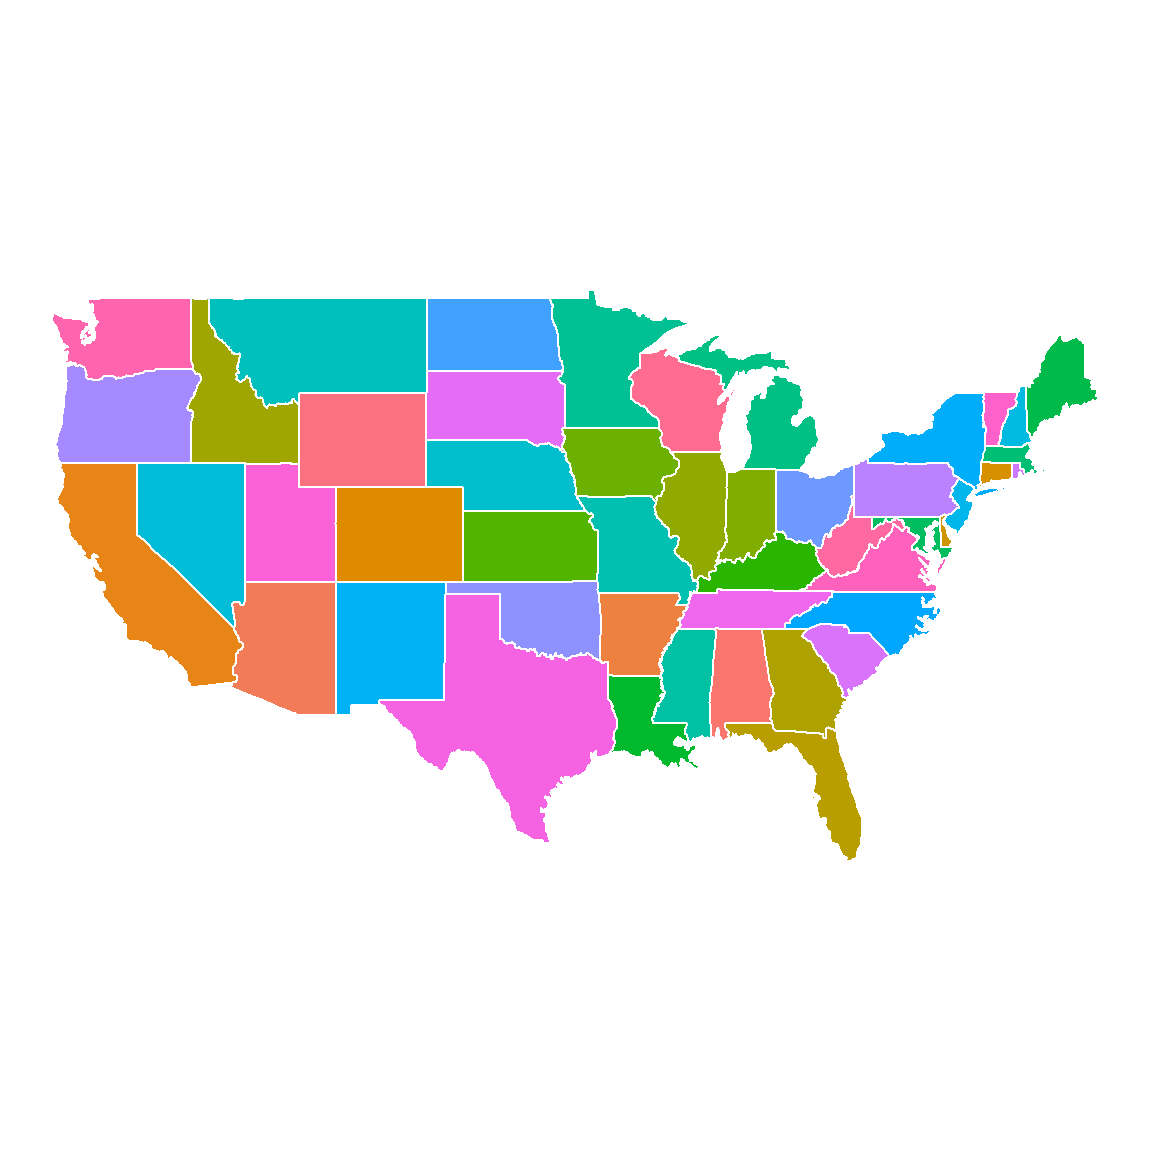
\includegraphics{lab1_files/figure-latex/unnamed-chunk-15-1.pdf}

\hypertarget{histogram}{%
\paragraph{Histogram}\label{histogram}}

A histogram provides the same information as the density plot but
provides a count instead of density on the x-axis.

\begin{Shaded}
\begin{Highlighting}[]
\FunctionTok{hist}\NormalTok{(new\_names}\SpecialCharTok{$}\NormalTok{school\_belif1, }\AttributeTok{col =} \StringTok{\textquotesingle{}lightgray\textquotesingle{}}\NormalTok{)}
\end{Highlighting}
\end{Shaded}

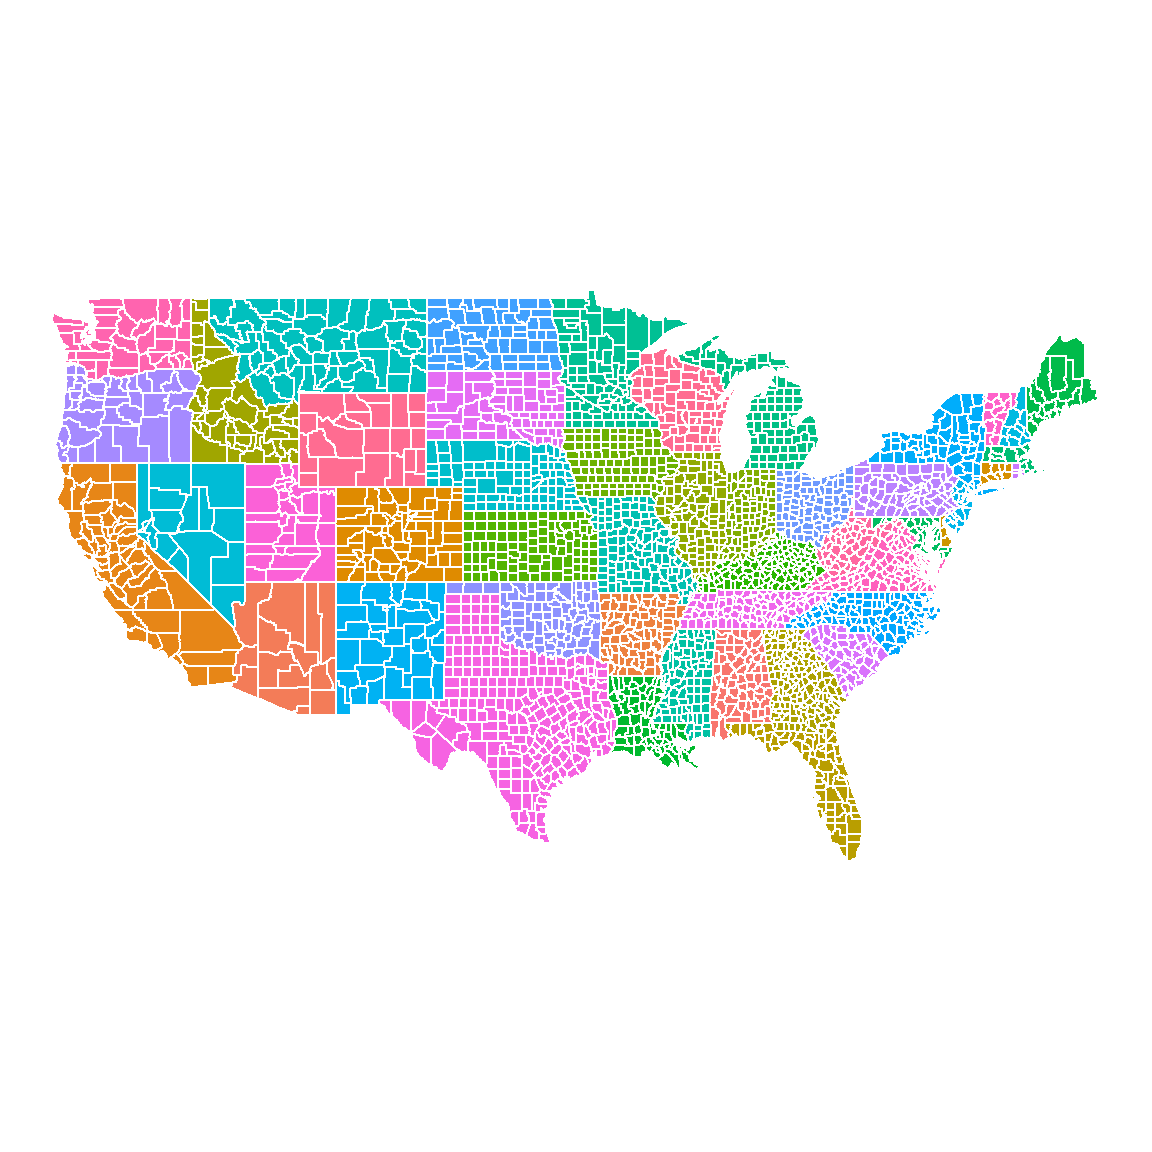
\includegraphics{lab1_files/figure-latex/unnamed-chunk-16-1.pdf}

\hypertarget{qq-plots}{%
\paragraph{QQ Plots}\label{qq-plots}}

QQ plot, or quantile-quantile plot, is a plot of the correlation between
a sample and the normal distribution. In a QQ plot, each observation is
plotted as a single dot. If the data are normal, the dots should form a
straight line. If the data are skewed, you will see either a downward
curve (negatively skewed) or upward curve (positively skewed).

\begin{Shaded}
\begin{Highlighting}[]
\FunctionTok{ggqqplot}\NormalTok{(new\_names}\SpecialCharTok{$}\NormalTok{school\_belif1)}
\end{Highlighting}
\end{Shaded}

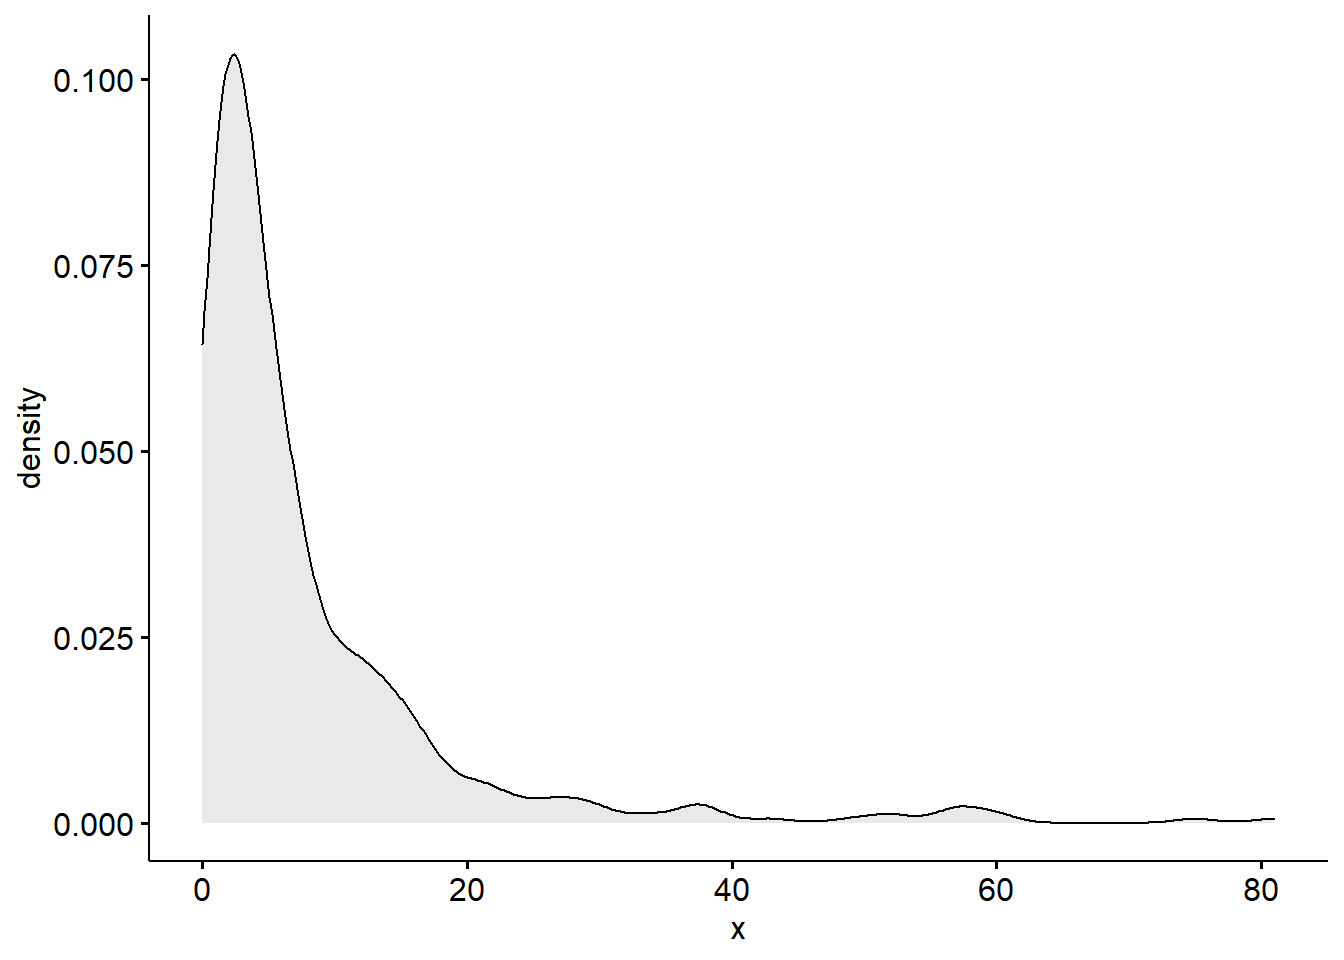
\includegraphics{lab1_files/figure-latex/unnamed-chunk-17-1.pdf}

As you can see in this QQ plot, there is an upward curve, which further
tells us that we have a positively skewed variable.

\hypertarget{box-plots}{%
\paragraph{Box Plots}\label{box-plots}}

Box plot can show us distributions, specifically the minimum, first
quartile, median, third quartile, and maximum.

\begin{Shaded}
\begin{Highlighting}[]
\NormalTok{new\_names }\SpecialCharTok{\%\textgreater{}\%} \CommentTok{\# }
  \FunctionTok{ggplot}\NormalTok{(}\FunctionTok{aes}\NormalTok{(}\AttributeTok{y =}\NormalTok{ school\_belif1)) }\SpecialCharTok{+}
  \FunctionTok{geom\_boxplot}\NormalTok{() }
\end{Highlighting}
\end{Shaded}

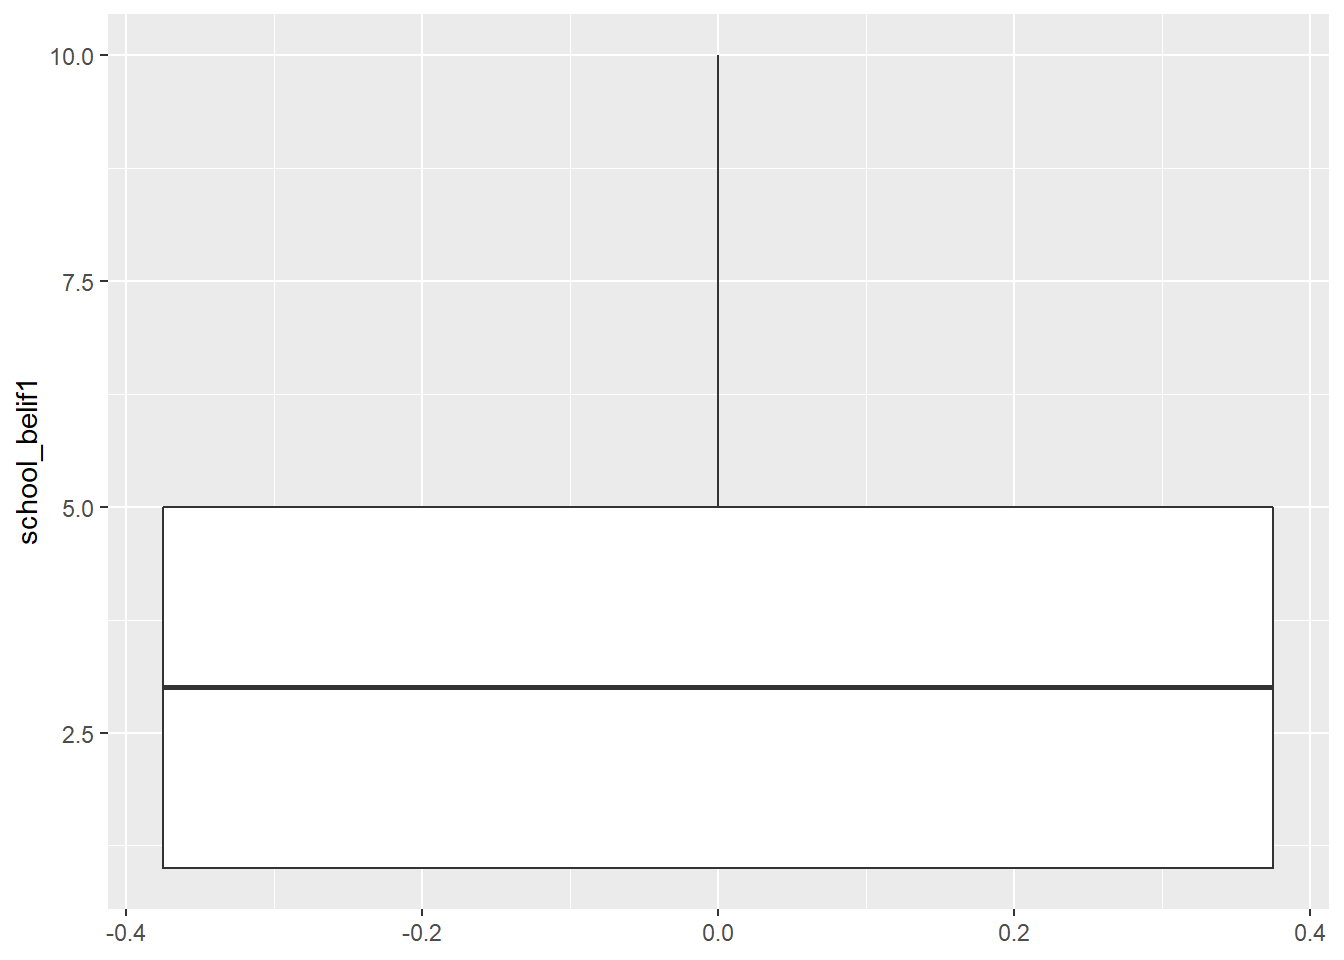
\includegraphics{lab1_files/figure-latex/unnamed-chunk-18-1.pdf}

\hypertarget{bivariate-scatterplots}{%
\paragraph{Bivariate Scatterplots}\label{bivariate-scatterplots}}

We can use \texttt{pairs()} to look at bivariate scatterplots. Do the
relationships look linear?:

\begin{Shaded}
\begin{Highlighting}[]
\FunctionTok{pairs}\NormalTok{(new\_names)}
\end{Highlighting}
\end{Shaded}

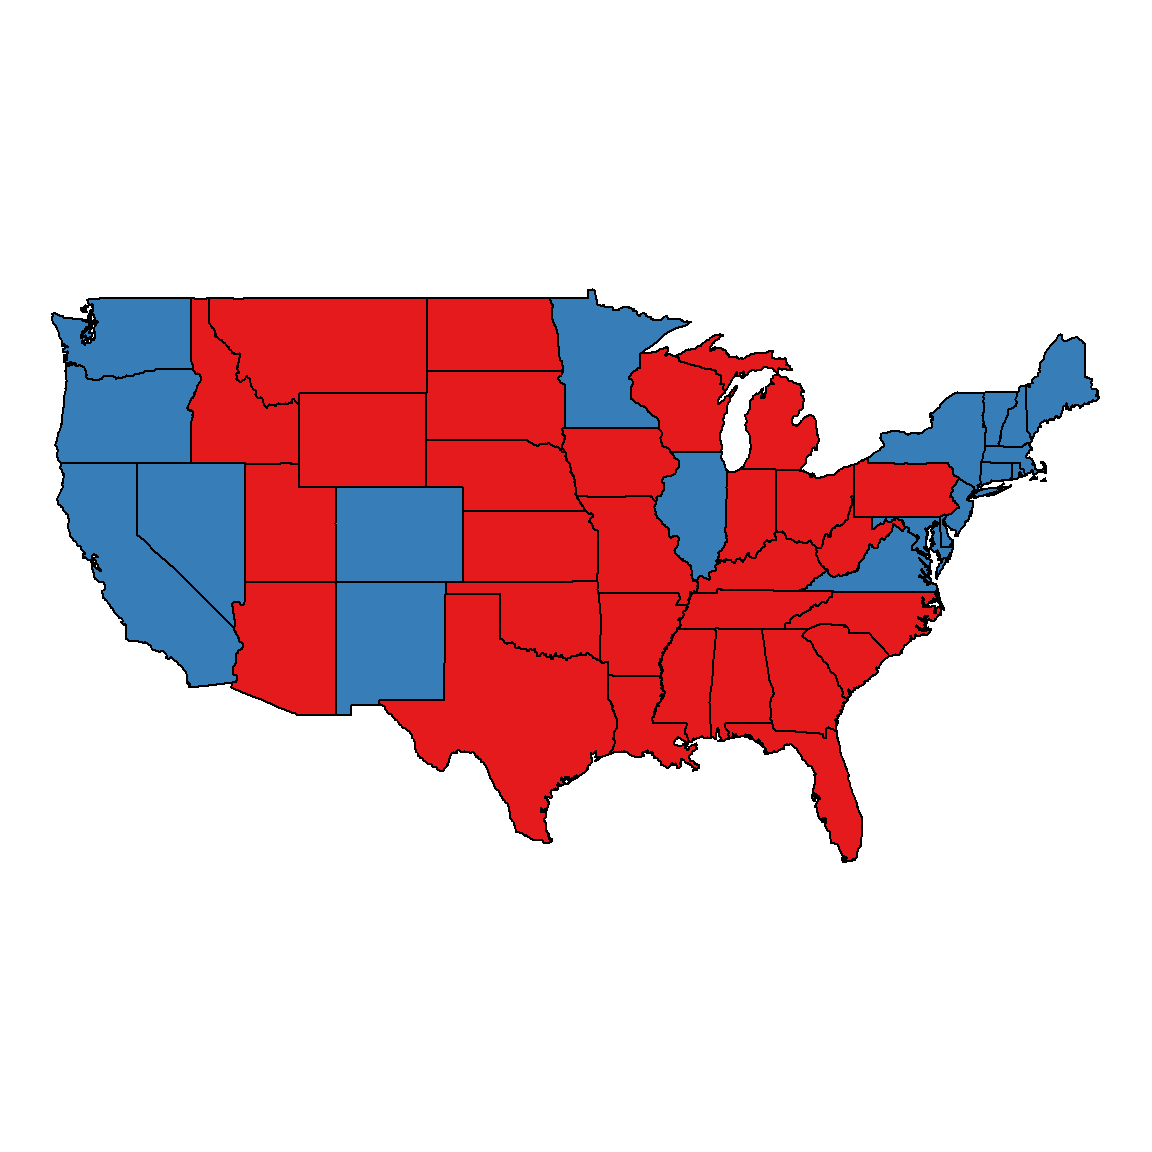
\includegraphics{lab1_files/figure-latex/unnamed-chunk-19-1.pdf}

\begin{Shaded}
\begin{Highlighting}[]
\CommentTok{\# Or we can look at individual scatterplots:}
\NormalTok{new\_names }\SpecialCharTok{\%\textgreater{}\%} 
  \FunctionTok{ggplot}\NormalTok{(}\FunctionTok{aes}\NormalTok{(school\_belif1, school\_belif2)) }\SpecialCharTok{+}
  \FunctionTok{geom\_point}\NormalTok{() }\SpecialCharTok{+}
  \FunctionTok{geom\_smooth}\NormalTok{(}\AttributeTok{method =} \StringTok{"lm"}\NormalTok{, }\AttributeTok{se =}\NormalTok{F) }\SpecialCharTok{+}
  \FunctionTok{theme\_minimal}\NormalTok{()}
\end{Highlighting}
\end{Shaded}

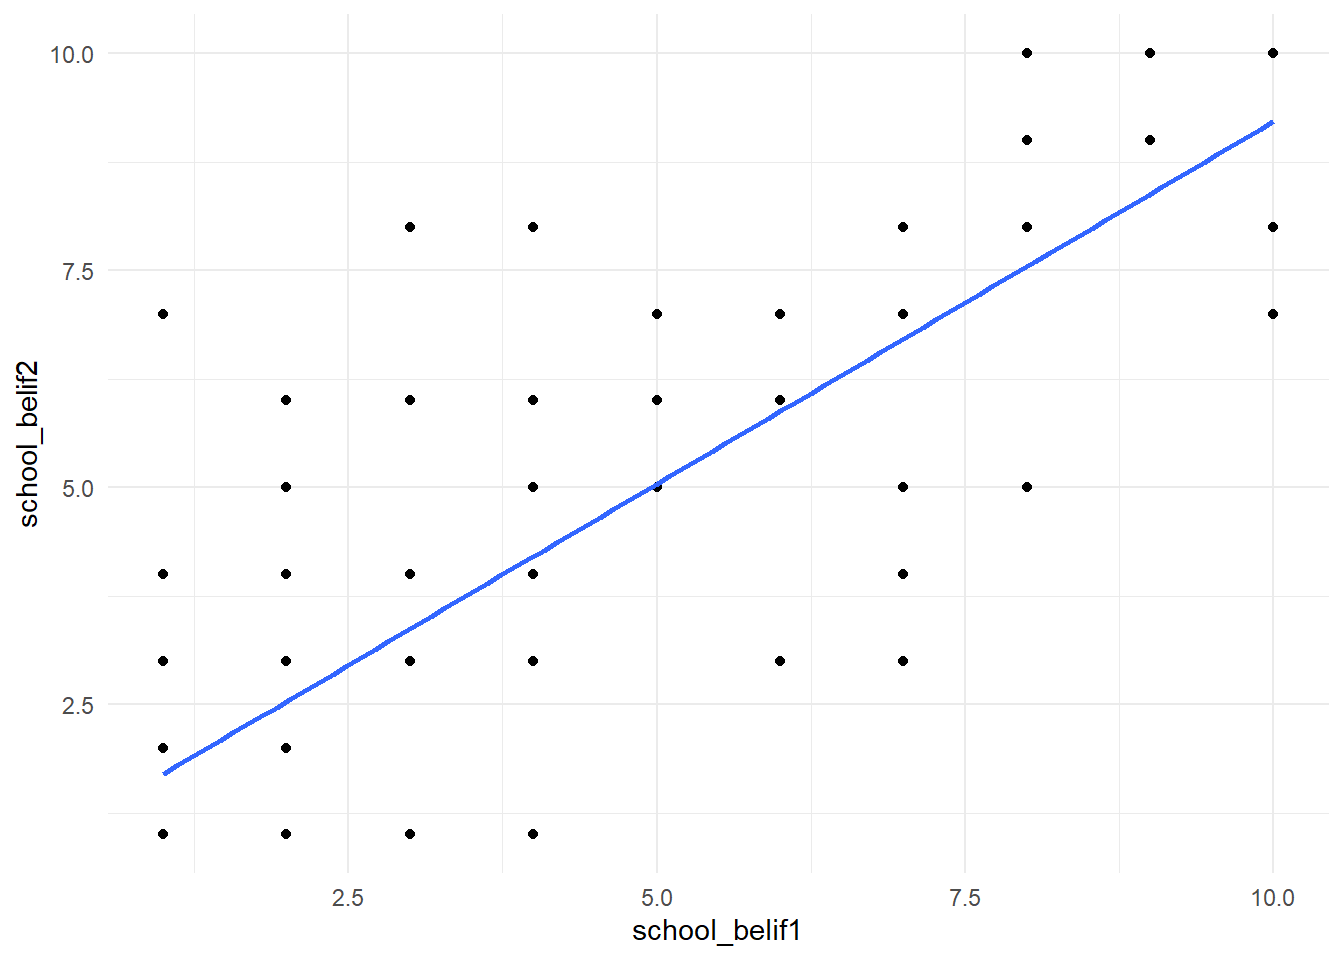
\includegraphics{lab1_files/figure-latex/unnamed-chunk-19-2.pdf}

We can also use \texttt{cor()} to look at bivariate correlations for the
entire data set (Note: Missing values are not allowed in correlation
analyses, use \texttt{drop\_na()} to do listwise deletion):

\begin{Shaded}
\begin{Highlighting}[]
\NormalTok{new\_names }\SpecialCharTok{\%\textgreater{}\%} 
  \FunctionTok{drop\_na}\NormalTok{() }\SpecialCharTok{\%\textgreater{}\%} \CommentTok{\#remove missing data}
  \FunctionTok{cor}\NormalTok{(}\AttributeTok{method =} \StringTok{"pearson"}\NormalTok{) }\SpecialCharTok{\%\textgreater{}\%} 
  \FunctionTok{round}\NormalTok{(}\DecValTok{2}\NormalTok{) }\CommentTok{\# round to 2 decimal places }
\end{Highlighting}
\end{Shaded}

\begin{verbatim}
##               school_motiv1 school_motiv2 school_motiv3 school_comp1
## school_motiv1          1.00          0.82          0.74         0.64
## school_motiv2          0.82          1.00          0.60         0.68
## school_motiv3          0.74          0.60          1.00         0.52
## school_comp1           0.64          0.68          0.52         1.00
## school_comp2           0.59          0.53          0.41         0.55
## school_comp3           0.61          0.69          0.57         0.71
## school_belif1          0.54          0.50          0.56         0.57
## school_belif2          0.63          0.55          0.58         0.67
## school_belif3          0.40          0.37          0.52         0.43
## female                 0.04          0.04          0.07         0.04
##               school_comp2 school_comp3 school_belif1 school_belif2
## school_motiv1         0.59         0.61          0.54          0.63
## school_motiv2         0.53         0.69          0.50          0.55
## school_motiv3         0.41         0.57          0.56          0.58
## school_comp1          0.55         0.71          0.57          0.67
## school_comp2          1.00         0.63          0.62          0.63
## school_comp3          0.63         1.00          0.65          0.68
## school_belif1         0.62         0.65          1.00          0.81
## school_belif2         0.63         0.68          0.81          1.00
## school_belif3         0.29         0.44          0.37          0.39
## female                0.00         0.01          0.04          0.00
##               school_belif3 female
## school_motiv1          0.40   0.04
## school_motiv2          0.37   0.04
## school_motiv3          0.52   0.07
## school_comp1           0.43   0.04
## school_comp2           0.29   0.00
## school_comp3           0.44   0.01
## school_belif1          0.37   0.04
## school_belif2          0.39   0.00
## school_belif3          1.00  -0.09
## female                -0.09   1.00
\end{verbatim}

\begin{Shaded}
\begin{Highlighting}[]
\CommentTok{\# A colorful plot:}
\NormalTok{f\_cor }\OtherTok{\textless{}{-}} \FunctionTok{cor}\NormalTok{(new\_names, }\AttributeTok{use =} \StringTok{"pairwise.complete.obs"}\NormalTok{)}
\FunctionTok{corrplot}\NormalTok{(f\_cor,}
         \AttributeTok{method=}\StringTok{"number"}\NormalTok{,}
         \AttributeTok{type =} \StringTok{"upper"}\NormalTok{)}
\end{Highlighting}
\end{Shaded}

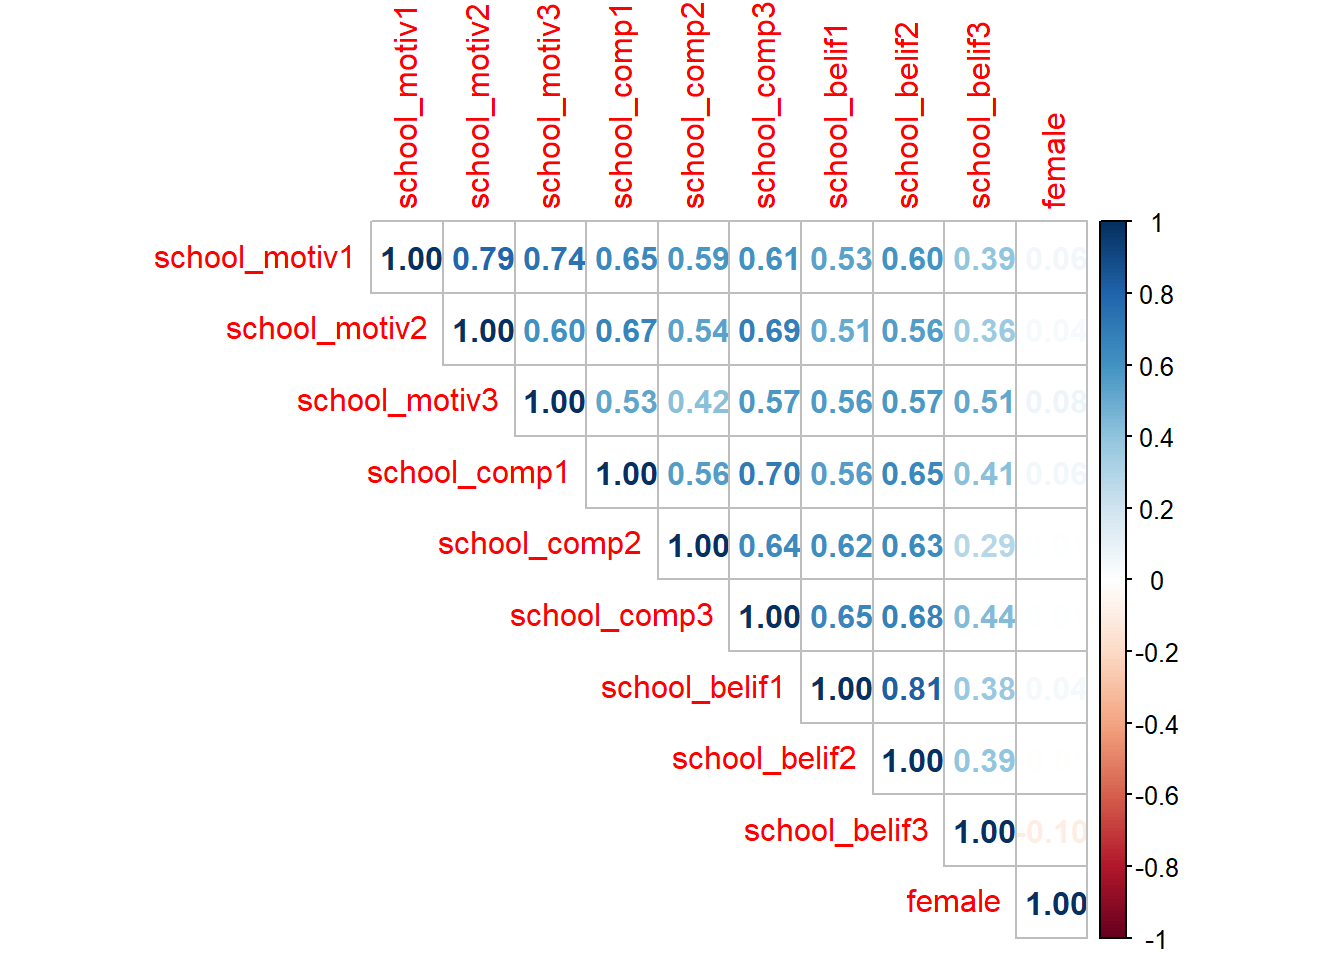
\includegraphics{lab1_files/figure-latex/unnamed-chunk-20-1.pdf}

\begin{Shaded}
\begin{Highlighting}[]
\CommentTok{\#Fun tip: \textasciigrave{}apa.cor.table()\textasciigrave{} creates an APA formated correlation matrix and saves it to your computer}
\CommentTok{\#apa.cor.table(physics, filename = "cor\_table.doc")}
\end{Highlighting}
\end{Shaded}

\hypertarget{skewness-and-kurtosis}{%
\paragraph{Skewness and Kurtosis}\label{skewness-and-kurtosis}}

One final thing to look are the skewness and kurtosis values in the
descriptive statistics provided earlier. There are many different
sources that provide different cut-off values, but as a general rule of
thumb, skewness and kurtosis values greater than +3/-3 indicate a
non-normal distribution. Positive skew values indicate positively skewed
variables and negative skew values indicate negatively skewed variables.
Positive values of kurtosis indicate leptokurtic distributions, or
higher peaks with taller tails than a normal distribution. Negative
values of kurtosis indicate platykurtic distributions, or flat peaks
with thin tails.

\begin{Shaded}
\begin{Highlighting}[]
\FunctionTok{describe}\NormalTok{(new\_names}\SpecialCharTok{$}\NormalTok{school\_belif1)}
\end{Highlighting}
\end{Shaded}

\begin{verbatim}
##    vars   n mean  sd median trimmed  mad min max range skew kurtosis   se
## X1    1 119 3.69 2.8      3    3.36 2.97   1  10     9 0.87    -0.58 0.26
\end{verbatim}

Here we can see that the \emph{skew} value is less than 3 and the
\emph{kurtosis} value is less than 3, indicating a normal distribution.

\begin{center}\rule{0.5\linewidth}{0.5pt}\end{center}

\hypertarget{references}{%
\subsection{References}\label{references}}

Hallquist, M. N. \& Wiley, J. F. (2018). MplusAutomation: An R Package
for Facilitating Large-Scale Latent Variable Analyses in Mplus.
Structural Equation Modeling, 25, 621-638. doi:
10.1080/10705511.2017.1402334.

Muthén, L.K. and Muthén, B.O. (1998-2017). Mplus User's Guide. Eighth
Edition. Los Angeles, CA: Muthén \& Muthén

R Core Team (2017). R: A language and environment for statistical
computing. R Foundation for Statistical Computing, Vienna, Austria. URL
\url{http://www.R-project.org/}

Wickham et al., (2019). Welcome to the tidyverse. Journal of Open Source
Software, 4(43), 1686, \url{https://doi.org/10.21105/joss.01686}

\textbf{Credits}

While I am creating these labs specifically for this W22 class, I am
incorporating some material from the previous TA's labs and his amazing
workshops: \href{https://garberadamc.github.io/project-site/}{Adam
Garber}. Big shout out to Adam for paving the way for us to switch over
from SPSS to R in GGSE and for providing resources to make Mplus
Automation more accessible to researchers. Please see Adam's website to
find more resources related to R studio and MplusAutomation.

\end{document}
